\section{La plataforma}

En este capítulo, se tratan los asuntos concernientes a la construcción de las funciones vitales del sistema, sobre las que
recaerán el control de los recursos, y la extensibilidad que pueda darsele a todo el proyecto.

\subsection{El gestor de paquetes \emph{packages}}

%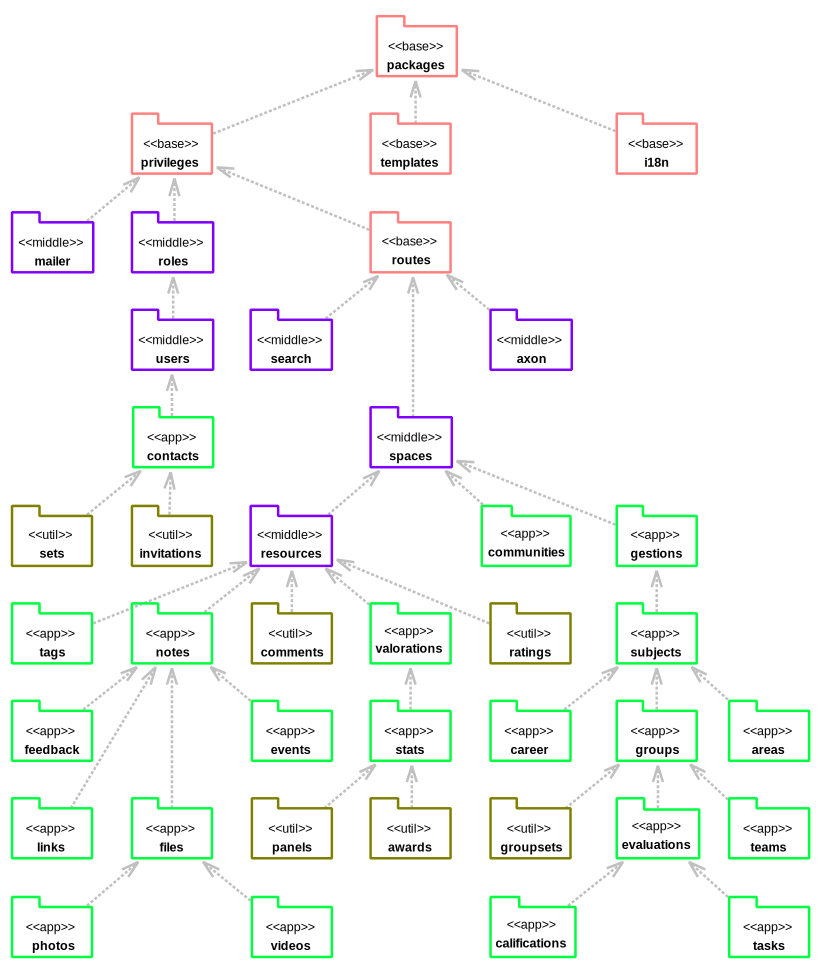
\includegraphics[scale=0.6]{../models/svg/yachay_packages.pdf}

\subsection{El manejo de privilegios \emph{privileges}}
\subsection{El manejo de rutas y navegación \emph{routes}}

\subsection{El sistema de plantillas \emph{templates}}

%\subsection{El motor de busqueda \emph{search}}
%\subsection{El sistema de traducciones \emph{i18n}}
%\subsection{La automatización de tareas \emph{cron}}
%\subsection{La cola de envio de correo \emph{mailer}}

\section{La conectitividad}

\section{La inteligencia colectiva \emph{axon}}

\section{Las personas}

\section{El espacio personal \emph{users}}
\section{El control de las funciones \emph{roles}}


\section{La red de contactos}

\subsection{Las redes sociales \emph{contacts}}
\subsection{Los círculos \emph{sets}}
\subsection{La propagación \emph{invitations}}


\section{El B-learning}

\subsection{Los sistemas de evaluación \emph{evaluations}}
\subsection{Las calificaciones \emph{califications}}
%\subsection{El trabajo para casa \emph{tasks}}

\section{Los recursos}

\subsection{Los componentes genéricos \emph{resources}}
\subsection{El recurso mas básico \emph{notes}}
\subsection{Los archivos en general \emph{files}}
\subsection{Los archivos especiales \emph{photos}, \emph{videos}}
\subsection{Los recursos espacio-temporales \emph{events}}
\subsection{La reenderizacion personalizada \emph{links}}
\subsection{Las sugerencias \emph{feedback}}


\section{Los aspectos 2.0}

\subsection{Los comentarios \emph{comments}}
\subsection{La calidad del recurso \emph{ratings}}
\subsection{Las nuevas interpretaciones \emph{tags}}
\subsection{Los sistemas de reputación \emph{valorations}}
%\subsection{Los refuerzos positivos \emph{awards}}


\section{Los sistemas de control}

\subsection{Los indicadores medibles \emph{stats}}
\subsection{El panel de control \emph{panels}}


